\documentclass[12pt, a4paper]{article}  

\usepackage{amsmath,amsfonts,amssymb,amsthm,mathtools} 

\usepackage{fontspec}        
\setmainfont{Roboto}       

\usepackage{unicode-math}    
\setmathfont{Asana Math}     

\usepackage{polyglossia}      
\newfontfamily{\cyrillicfont}{Roboto}
\setdefaultlanguage{russian} 
\setotherlanguage{english}    

\usepackage{graphicx}

\title{Уютный факультатив по \LaTeX. Домашнее задание №1 }
\author{Дарья Решетникова}
\date{\today}

\begin{document} 


\maketitle

\section{10 фактов обо мне}

\begin{enumerate}
	\item Зовут меня Даша Решетникова, родилась в Москве и живу здесь всю свою жизнь.
	\item Почти окончила музыкальную школу по классу фортепиано, но бросила это занятие, о чем сейчас периодически жалею.
	\item Люблю путешествовать и открывать для себя новые места. Но, есть города, в которые  готова возвращаться снова и снова, например, в Прагу.
	\item Категорически не жалею о принятом решении поступить на Эконом в РАНХ, а не в ВШЭ.
	\item Некоторые личности видят в моей внешности сходство с Джинни Уизли, что неимоверно меня раздражает\label{nomer1}.
	\item Если хочешь остаться в живых - никогда не говори мне о том, что я рассказала в пункте \ref{nomer1}.
	\item Многие близкие друзья округляют глаза и грозятся засадить меня под домашний арест, когда узнают, что я не смотрела многие культовые фильмы.
	\item Люблю людей, которые открывают мне/со мной новые горизонты, показывают/рассказывают интересные вещи.
	\item У меня никогда не было домашнего животного, кроме рыбок, которые прожили очень недолго, к сожалению.
	\item Люблю Москву, особенно летом, особенно вечером/ночью. Прогулки по улочкам с вкусным кофе и приятной беседой в хорошей компании вдохновляют.
\end{enumerate}

\subsection{Фотография}

\begin{figure}[h]
	\centering
	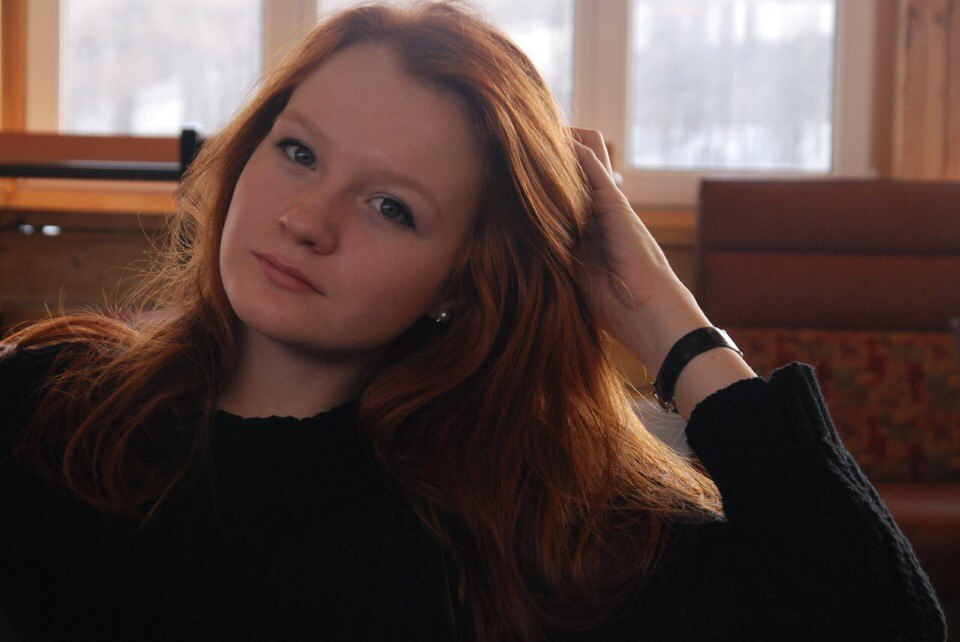
\includegraphics[scale=0.3]{image1.jpg}
\end{figure}

\section{Формулы}

 \begin{equation}
 \lim\limits_{x \to 0} \frac{\sin x}{x} = 1 \label{æ}
 \end{equation}
	
\begin{equation}
 \left\lbrace \beta_{1,0}, \beta_{2,0} : F = \frac{1}{2} \cdot \left(\frac{t^2_1 + t^2_2 - \hat{\rho_{t_1,t_2}} \cdot t_1 \cdot t_2 }{1 - \hat{\rho_{t_1,t_2}}}\right)  < 3,00\right\rbrace  \label{ææ}
\end{equation}


\begin{multline}
f(x) = f(a) + \frac{f`(a)}{1!} \cdot (x-a) + \frac{f``(a)}{2!} \cdot (x-a)^2 + \frac{f```(a)}{3!} \cdot (x-a)^3 + \\
\cdots + \frac{f^{(n)}(a)}{n!} \cdot (x-a)^n + \cdots \label{æææ}
\end{multline}

\begin{equation}
\int_{X} f(x) \mu(dx) = \sum_{i=1}^{n} f_i \mu(F_i) \label{ææææ}
\end{equation}
	
\begin{equation} H(f) = 
 \begin{bmatrix}
	\frac{\partial^2f}{\partial x^2_1} & \frac{\partial^2 f}{\partial x_1 \partial x_2} & \cdots & \frac{\partial^2 f}{\partial x_1 \partial x_n} \\
	\frac{\partial^2 f}{\partial x_2 \partial x_1} & \frac{\partial^2 f}{\partial x^2_2} & \cdots & \frac{\partial^2 f}{\partial x_2 \partial x_n} \\
	\vdots  & \vdots  & \ddots & \vdots  \\
	\frac{\partial^2 f}{\partial x_n \partial x_1} & \frac{\partial^2 f}{\partial x_n \partial x_2} & \cdots & \frac{\partial^2 f}{\partial x^2_n} \label{æææææ}
\end{bmatrix}
\end{equation}

\subsection{Краткое описание}
Формула \ref{æ} - первый замечательный предел. \\
Формула \ref{ææ} - доверительная область для нескольких (двух) коэффициентов.\\
Формула \ref{æææ} - формула разложения функции в степенной ряд - ряд Тейлора.\\
Формула \ref{ææææ} представляет собой Интеграл Лебега.\\
Формула \ref{æææææ} - матрица Гессе.



\end{document}
